% \VignetteIndexEntry{ A Short Introduction to the caret Package}
% \VignetteDepends{caret}
% \VignettePackage{caret}
\documentclass[12pt]{article}
\usepackage{colortbl}
\usepackage{amsmath}
\usepackage[pdftex]{graphicx}
\usepackage{color}
\usepackage{xspace}
\usepackage{fancyvrb}
\usepackage{fancyhdr}
\usepackage[
         colorlinks=true,
         linkcolor=blue,
         citecolor=blue,
         urlcolor=blue]
         {hyperref}

\usepackage{Sweave}

%%%%%%%%%%%%%%%%%%%%%%%%%%%%%%%%%%%%%%%%%%%%%%%%%%%%%%%%%%%%%%%%%%

% define new colors for use
\definecolor{darkgreen}{rgb}{0,0.6,0}
\definecolor{darkred}{rgb}{0.6,0.0,0}
\definecolor{lightbrown}{rgb}{1,0.9,0.8}
\definecolor{brown}{rgb}{0.6,0.3,0.3}
\definecolor{darkblue}{rgb}{0,0,0.8}
\definecolor{darkmagenta}{rgb}{0.5,0,0.5}

%%%%%%%%%%%%%%%%%%%%%%%%%%%%%%%%%%%%%%%%%%%%%%%%%%%%%%%%%%%%%%%%%%

\newcommand{\bld}[1]{\mbox{\boldmath $#1$}}
\newcommand{\shell}[1]{\mbox{$#1$}}
\renewcommand{\vec}[1]{\mbox{\bf {#1}}}
 \newcommand{\codeheading}[1]{\mbox{\color{darkblue}\texttt{#1}}}
\newcommand{\code}[1]{\mbox{\footnotesize\color{darkblue}\texttt{#1}}}
\newcommand{\pkg}[1]{{\fontseries{b}\selectfont #1}}
\renewcommand{\pkg}[1]{{\textsf{#1}}}

\newcommand{\ReallySmallSpacing}{\renewcommand{\baselinestretch}{.6}\Large\normalsize}
\newcommand{\SmallSpacing}{\renewcommand{\baselinestretch}{1.1}\Large\normalsize}

\providecommand{\SetAlgoLined}{\SetLine}

\newcommand{\halfs}{\frac{1}{2}}

\setlength{\oddsidemargin}{-.25 truein}
\setlength{\evensidemargin}{0truein}
\setlength{\topmargin}{-0.2truein}
\setlength{\textwidth}{7 truein}
\setlength{\textheight}{8.5 truein}
\setlength{\parindent}{0truein}
\setlength{\parskip}{0.10truein}


\DefineVerbatimEnvironment{Sinput}{Verbatim}{fontshape=sl,formatcom=\color{darkblue}} 
\fvset{listparameters={\setlength{\topsep}{0pt}}}
\renewenvironment{Schunk}{\vspace{\topsep}}{\vspace{\topsep}}

\fvset{fontsize=\footnotesize}
 

%%%%%%%%%%%%%%%%%%%%%%%%%%%%%%%%%%%%%%%%%%%%%%%%%%%%%%%%%%%%%%%%%%
\pagestyle{fancy}
\lhead{}
\chead{The {\tt caret} Package}
\rhead{}
\lfoot{}
\cfoot{}
\rfoot{\thepage}
\renewcommand{\headrulewidth}{1pt}
\renewcommand{\footrulewidth}{1pt}
%%%%%%%%%%%%%%%%%%%%%%%%%%%%%%%%%%%%%%%%%%%%%%%%%%%%%%%%%%%%%%%%%%

\title{A Short Introduction to the \pkg{caret} Package}
\author{Max Kuhn \\ max.kuhn@pfizer.com}


\begin{document}
\Sconcordance{concordance:caret.tex:caret.Rnw:%
1 33 1 49 0 1 17 122 1 1 5 397 1 4 0 10 1 4 0 54 1}


\maketitle

\thispagestyle{empty}
  
\vspace{.2in}

\renewcommand{\baselinestretch}{1}
 
	
	


The \pkg{caret} package (short for
{\bf{\color{blue}{c}}}lassification {\bf{\color{blue}{a}}}nd
{\bf{\color{blue}{re}}}gression {\bf{\color{blue}{t}}}raining)
contains functions to streamline the model training process for
complex regression and classification problems. The package utilizes a
number of R packages but tries not to load them all at package
start-up\footnote{By adding formal package dependencies, the package
  startup time can be greatly decreased}. The package ``suggests''
field includes  27 packages. \pkg{caret} loads
packages as needed and assumes that they are installed. Install
\pkg{caret} using  
\begin{Schunk}
\begin{Sinput}
> install.packages("caret", dependencies = c("Depends", "Suggests"))
\end{Sinput}
\end{Schunk}
to ensure that all the needed packages are installed.

The {\bf main help pages} for the package are at:
\begin{center}
\url{http://caret.r-forge.r-project.org/}
\end{center}
Here, there are extended examples and a large amount of information
that previously found in the package vignettes. 


\pkg{caret} has several functions that attempt to streamline the model building and evaluation process, as well as feature selection and other techniques. 

One of the primary tools in the package is the \code{train} function which can be used to
\begin{itemize}
   \item evaluate, using resampling, the effect of model tuning parameters on performance
   \item choose the ``optimal'' model across these parameters 
   \item estimate model performance from a training set
\end{itemize}

More formally:

  \begin{center}  
    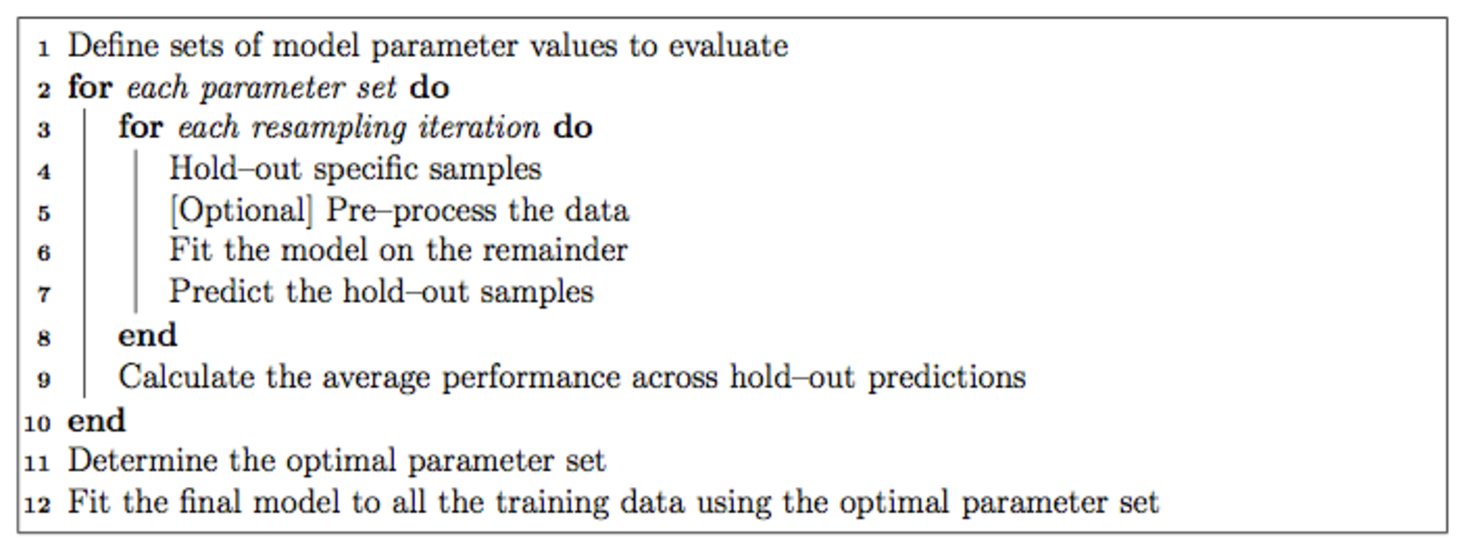
\includegraphics[clip, width = .9\textwidth]{train_algo}
  \end{center}

There are options for customizing almost every step of this process (e.g. resampling technique, choosing the optimal parameters etc). To demonstrate this function, the Sonar data from the \pkg{mlbench} package will be used.

The Sonar data consist of 208 data points collected on 60 predictors. The goal is to predict the two classes (\texttt{M} for metal cylinder or \texttt{R} for rock).

First, we split the data into two groups: a training set and a test set. To do this, the \code{createDataPartition} function is used:
\begin{Schunk}
\begin{Sinput}
> library(caret)
> library(mlbench)
> data(Sonar)
> set.seed(107)
> inTrain <- createDataPartition(y = Sonar$Class, 
+                                ## the outcome data are needed
+                                p = .75, 
+                                ## The percentage of data in the 
+                                ## training set
+                                list = FALSE)
>                                ## The format of the results
> 
> ## The output is a set of integers for the rows of Sonar 
> ## that belong in the training set.
> str(inTrain)
\end{Sinput}
\begin{Soutput}
 int [1:157, 1] 1 2 3 6 7 9 10 11 12 13 ...
 - attr(*, "dimnames")=List of 2
  ..$ : NULL
  ..$ : chr "Resample1"
\end{Soutput}
\end{Schunk}
By default, \code{createDataPartition} does a stratified random split of the data. To partition the data:

\begin{Schunk}
\begin{Sinput}
> training <- Sonar[ inTrain,]
> testing  <- Sonar[-inTrain,]
> nrow(training)
\end{Sinput}
\begin{Soutput}
[1] 157
\end{Soutput}
\begin{Sinput}
> nrow(testing)
\end{Sinput}
\begin{Soutput}
[1] 51
\end{Soutput}
\end{Schunk}

To tune a model using Algorithm \ref{A:tune}, the \code{train} function can be used. More details on this function can be found at:
\begin{center}
\url{http://caret.r-forge.r-project.org/training.html}
\end{center}
Here, a partial least squares discriminant analysis (PLSDA) model will be tuned over the number of PLS components that should be retained. The most basic syntax to do this is:
\begin{Schunk}
\begin{Sinput}
> plsFit <- train(Class ~ ., 
+                 data = training,
+                 method = "pls",
+                 ## Center and scale the predictors for the training 
+                 ## set and all future samples.
+                 preProc = c("center", "scale"))
\end{Sinput}
\end{Schunk}
However, we would probably like to customize it in a few ways:
\begin{itemize}
\item expand the set of PLS models that the function evaluates. By default, the function will tune over three values of each tuning parameter. 
\item the type of resampling used. The simple bootstrap is used by default. We will have the function use three repeats of 10--fold cross--validation.
\item the methods for measuring performance. If unspecified, overall accuracy and the Kappa statistic are computed. For regression models, root mean squared error and $R^2$ are computed. Here, the function will be altered to estimate the area under the ROC curve, the sensitivity and specificity 
\end{itemize}
To change the candidate values of the tuning parameter, either of the \code{tuneLength} or \code{tuneGrid} arguments can be used. The \code{train} function can generate a candidate set of parameter values and the \code{tuneLength} argument controls how many are evaluated. In the case of PLS, the function uses a sequence of integers from 1 to \code{tuneLength}. If we want to evaluate all integers between 1 and 15, setting \code{tuneLength = 15} would achieve this. The \code{tuneGrid} argument is used when specific values are desired. A data frame is used where each row is a tuning parameter setting and each column is a tuning parameter. An example is used below to illustrate this. 

The syntax for the model would then be:
\begin{Verbatim}[fontshape=sl,formatcom=\color{darkblue},fontsize=\footnotesize,commandchars=\\\{\}]
> plsFit <- train(Class ~ ., 
+                 data = training,
+                 method = "pls",
+                 \textcolor{red}{tuneLength = 15},
+                 preProc = c("center", "scale"))                     
\end{Verbatim}

To modify the resampling method, a \code{trainControl} function is used. The option \code{method} controls the type of resampling and defaults to \code{"boot"}. Another method, \code{"repeatedcv"}, is used to specify repeated $K$--fold cross--validation (and the argument \code{repeats} controls the number of repetitions). $K$ is controlled by the \code{number} argument and defaults to 10. The new syntax is then:
\begin{Verbatim}[fontshape=sl,formatcom=\color{darkblue},fontsize=\footnotesize,commandchars=\\\{\}]
> \textcolor{red}{ctrl <- trainControl(method = "repeatedcv",}
+ \textcolor{red}{                     repeats = 3)}
> plsFit <- train(Class ~ ., 
+                 data = training,
+                 method = "pls",
+                 tuneLength = 15,
+                 \textcolor{red}{trControl = ctrl},
+                 preProc = c("center", "scale"))                     
\end{Verbatim}
Finally, to choose different measures of performance, additional arguments are given to \code{trainControl}. The \code{summaryFunction} argument is used to pas in a function that takes the observed and predicted values and estimate some measure of performance. Two such functions are already included in the package: \code{defaultSummary} and \code{twoClassSummary}. The latter will compute measures specific to two--class problems, such as the area under the ROC curve, the sensitivity and specificity. Since the ROC curve is based on the predicted class probabilities (which are not computed automatically), another option is required. The \code{classProbs = TRUE} option is used to include these calculations. 

Lastly, the function will pick the tuning parameters associated with the best results. Since we are using custom performance measures, the criterion that should be optimized must also be specified. In the call to \code{train}, we can use \code{metric = "ROC"} to do this.

The final model fit would then be:
\begin{Verbatim}[fontshape=sl,formatcom=\color{darkblue},fontsize=\footnotesize,commandchars=\\\{\}]
> set.seed(123) 
> ctrl <- trainControl(method = "repeatedcv",
+                      repeats = 3,
+ \textcolor{red}{                     classProbs = TRUE},
+ \textcolor{red}{                     summaryFunction = twoClassSummary})
> plsFit <- train(Class ~ ., 
+                 data = training,
+                 method = "pls",
+                 tuneLength = 15,
+                 trControl = ctrl,
+                 \textcolor{red}{metric = "ROC"},
+                 preProc = c("center", "scale"))                     
\end{Verbatim}
\begin{Schunk}
\begin{Sinput}
> plsFit
\end{Sinput}
\begin{Soutput}
Partial Least Squares 

157 samples
 60 predictor
  2 classes: 'M', 'R' 

Pre-processing: centered (60), scaled (60) 
Resampling: Cross-Validated (10 fold, repeated 3 times) 
Summary of sample sizes: 142, 141, 141, 141, 142, 142, ... 
Resampling results across tuning parameters:

  ncomp  ROC        Sens       Spec     
   1     0.8135582  0.7120370  0.7172619
   2     0.8713211  0.7782407  0.8130952
   3     0.8660962  0.7699074  0.8339286
   4     0.8660136  0.7740741  0.7714286
   5     0.8504216  0.7532407  0.7845238
   6     0.8352679  0.7574074  0.8035714
   7     0.8093419  0.7296296  0.7791667
   8     0.8152116  0.7259259  0.7744048
   9     0.8194362  0.7291667  0.7517857
  10     0.8254299  0.7296296  0.7654762
  11     0.8303241  0.7416667  0.7702381
  12     0.8275298  0.7458333  0.7738095
  13     0.8295387  0.7337963  0.7744048
  14     0.8225364  0.7375000  0.7833333
  15     0.8150463  0.7337963  0.7744048

ROC was used to select the optimal model using  the largest value.
The final value used for the model was ncomp = 2. 
\end{Soutput}
\end{Schunk}
In this output the grid of results are the average resampled estimates of performance. The note at the bottom tells the user that  PLS components were found to be optimal. Based on this value, a final PLS model is fit to the whole data set using this specification and this is the model that is used to predict future samples.

The package has several functions for visualizing the results. One method for doing this is the \code{plot} function for \code{train} objects. The command \code{plot(plsFit)} produced the results seen in Figure \ref{F:pls} and shows the relationship between the resampled performance values and the number of PLS components. 

\setkeys{Gin}{width=.65\textwidth}
\begin{figure}
  \begin{center}  
\includegraphics{caret-baPlot}
    \caption{
      \code{plot(plsFit)} shows
      the relationship between the number of
      PLS components and the resampled
      estimate of the area under the ROC curve.  }
    \label{F:pls}         
  \end{center}
\end{figure}   


To predict new samples, \code{predict.train} can be used. For classification models, the default behavior is to calculated the predicted class. Using the option \code{type = "prob"} can be used to compute class probabilities from the model. For example:
\begin{Schunk}
\begin{Sinput}
> plsClasses <- predict(plsFit, newdata = testing)
> str(plsClasses)
\end{Sinput}
\begin{Soutput}
 Factor w/ 2 levels "M","R": 2 1 1 2 1 2 2 2 2 2 ...
\end{Soutput}
\begin{Sinput}
> plsProbs <- predict(plsFit, newdata = testing, type = "prob")
> head(plsProbs)
\end{Sinput}
\begin{Soutput}
           M         R
4  0.3762529 0.6237471
5  0.5229047 0.4770953
8  0.5839468 0.4160532
16 0.3660142 0.6339858
20 0.7351013 0.2648987
25 0.2135788 0.7864212
\end{Soutput}
\end{Schunk}

\pkg{caret} contains a function to compute the confusion matrix and associated statistics for the model fit:
\begin{Schunk}
\begin{Sinput}
> confusionMatrix(data = plsClasses, testing$Class)
\end{Sinput}
\begin{Soutput}
$positive
[1] "M"

$table
          Reference
Prediction  M  R
         M 20  7
         R  7 17

$overall
      Accuracy          Kappa  AccuracyLower  AccuracyUpper   AccuracyNull 
   0.725490196    0.449074074    0.582552477    0.841072735    0.529411765 
AccuracyPValue  McnemarPValue 
   0.003346986    1.000000000 

$byClass
         Sensitivity          Specificity       Pos Pred Value 
           0.7407407            0.7083333            0.7407407 
      Neg Pred Value            Precision               Recall 
           0.7083333            0.7407407            0.7407407 
                  F1           Prevalence       Detection Rate 
           0.7407407            0.5294118            0.3921569 
Detection Prevalence    Balanced Accuracy 
           0.5294118            0.7245370 

$mode
[1] "sens_spec"

$dots
list()

attr(,"class")
[1] "confusionMatrix"
\end{Soutput}
\end{Schunk}

To fit an another model to the data, \code{train} can be invoked with minimal changes. Lists of models available can be found at:
\begin{center}
\url{http://caret.r-forge.r-project.org/modelList.html}

\url{http://caret.r-forge.r-project.org/bytag.html}
\end{center}
For example, to fit a regularized discriminant model to these data, the following syntax can be used:
\begin{Schunk}
\begin{Sinput}
> ## To illustrate, a custom grid is used
> rdaGrid = data.frame(gamma = (0:4)/4, lambda = 3/4)
> set.seed(123)                    
> rdaFit <- train(Class ~ ., 
+                 data = training,
+                 method = "rda",
+                 tuneGrid = rdaGrid,
+                 trControl = ctrl,
+                 metric = "ROC")
> rdaFit
\end{Sinput}
\begin{Soutput}
Regularized Discriminant Analysis 

157 samples
 60 predictor
  2 classes: 'M', 'R' 

No pre-processing
Resampling: Cross-Validated (10 fold, repeated 3 times) 
Summary of sample sizes: 142, 141, 141, 141, 142, 142, ... 
Resampling results across tuning parameters:

  gamma  ROC        Sens       Spec     
  0.00   0.8448826  0.7884259  0.7625000
  0.25   0.8860119  0.8060185  0.8035714
  0.50   0.8851190  0.8097222  0.7666667
  0.75   0.8685847  0.7745370  0.7529762
  1.00   0.7563823  0.6615741  0.6803571

Tuning parameter 'lambda' was held constant at a value of 0.75
ROC was used to select the optimal model using  the largest value.
The final values used for the model were gamma = 0.25 and lambda = 0.75. 
\end{Soutput}
\begin{Sinput}
> rdaClasses <- predict(rdaFit, newdata = testing)
> confusionMatrix(rdaClasses, testing$Class)
\end{Sinput}
\begin{Soutput}
$positive
[1] "M"

$table
          Reference
Prediction  M  R
         M 22  5
         R  5 19

$overall
      Accuracy          Kappa  AccuracyLower  AccuracyUpper   AccuracyNull 
  0.8039215686   0.6064814815   0.6688426487   0.9017565835   0.5294117647 
AccuracyPValue  McnemarPValue 
  0.0000434105   1.0000000000 

$byClass
         Sensitivity          Specificity       Pos Pred Value 
           0.8148148            0.7916667            0.8148148 
      Neg Pred Value            Precision               Recall 
           0.7916667            0.8148148            0.8148148 
                  F1           Prevalence       Detection Rate 
           0.8148148            0.5294118            0.4313725 
Detection Prevalence    Balanced Accuracy 
           0.5294118            0.8032407 

$mode
[1] "sens_spec"

$dots
list()

attr(,"class")
[1] "confusionMatrix"
\end{Soutput}
\end{Schunk}

How do these models compare in terms of their resampling results? The \code{resamples} function can be used to collect, summarize and contrast the resampling results. Since the random number seeds were initialized to the same value prior to calling \code{train}, the same folds were used for each model. To assemble them:
\begin{Schunk}
\begin{Sinput}
> resamps <- resamples(list(pls = plsFit, rda = rdaFit))
> summary(resamps)
\end{Sinput}
\begin{Soutput}
Call:
summary.resamples(object = resamps)

Models: pls, rda 
Number of resamples: 30 

ROC 
      Min. 1st Qu. Median   Mean 3rd Qu. Max. NA's
pls 0.5397  0.8333 0.8672 0.8713  0.9509    1    0
rda 0.6984  0.8398 0.9028 0.8860  0.9787    1    0

Sens 
      Min. 1st Qu. Median   Mean 3rd Qu. Max. NA's
pls 0.3333  0.7500 0.7778 0.7782  0.8750    1    0
rda 0.4444  0.6875 0.8750 0.8060  0.8889    1    0

Spec 
      Min. 1st Qu. Median   Mean 3rd Qu. Max. NA's
pls 0.5000  0.7143 0.8571 0.8131  0.9688    1    0
rda 0.1429  0.7232 0.8571 0.8036  0.8571    1    0
\end{Soutput}
\end{Schunk}
There are several functions to visualize these results. For example, a Bland--Altman type plot can be created using \code{xyplot(resamps, what = "BlandAltman")} (see Figure \ref{F:BA}). The results look similar. Since, for each resample, there are paired results a paired $t$--test can be used to assess whether there is a difference in the average resampled area under the ROC curve. The \code{diff.resamples} function can be used to compute this:
\begin{Schunk}
\begin{Sinput}
> diffs <- diff(resamps)